\documentclass[../main.tex]{subfiles}

\begin{document}

\section{Resultados}

En este apartado se muestran los resultados obtenidos en las pruebas diseñadas en la sección anterior.

Cabe mencionar que todos los valores que se presentan están en microsegundos.

%----------------------------------------------------------------------------------
\subsection{Tiempo máximo con interrupciones inhibidas}

Los resultados agregados en una tabla son los siguientes:

% Please add the following required packages to your document preamble:
% \usepackage{multirow}
\begin{table}[htp]
\begin{tabular}{|c|c|c|c|c|c|c|c|c|}
\hline
\multicolumn{9}{|c|}{\textbf{irqsoff}}                                                                                                                               \\ \hline
\multirow{2}{*}{\textbf{nº workers}} & \multicolumn{4}{c|}{\textit{\textbf{No Forced Preemption}}}   & \multicolumn{4}{c|}{\textit{\textbf{Full Preemption}}}        \\ \cline{2-9} 
                                     & \textbf{Avg} & \textbf{Max} & \textbf{Min} & \textbf{Std Dev} & \textbf{Avg} & \textbf{Max} & \textbf{Min} & \textbf{Std Dev} \\ \hline
\textit{4}                           & 1024,8       & 4626         & 568          & 1265,70          & 887          & 1034         & 800          & 67,19            \\ \hline
\textit{7}                           & 820,3        & 980          & 758          & 66,55            & 1139         & 1260         & 999          & 82,39            \\ \hline
\textit{10}                          & 902,5        & 1025         & 857          & 50,91            & 1247,9       & 1339         & 1170         & 51,85            \\ \hline
\textit{13}                          & 974,5        & 1187         & 830          & 104,65           & 1301,8       & 1552         & 1209         & 122,37           \\ \hline
\textit{16}                          & 913,8        & 1058         & 800          & 87,10            & 1250,8       & 1633         & 1082         & 180,17           \\ \hline
\textit{19}                          & 946          & 1124         & 845          & 90,81            & 1208,9       & 1299         & 1114         & 60,86            \\ \hline
\textit{22}                          & 977          & 1050         & 872          & 47,65            & 1209,4       & 1377         & 1105         & 89,49            \\ \hline
\textit{25}                          & 930,6        & 1009         & 844          & 54,34            & 1300,9       & 1695         & 1121         & 155,78           \\ \hline
\textit{28}                          & 946,7        & 1024         & 851          & 64,50            & 1192         & 1331         & 1124         & 72,48            \\ \hline
\textit{31}                          & 987,9        & 1146         & 845          & 87,51            & 1207,3       & 1315         & 1033         & 98,91            \\ \hline
\textit{34}                          & 937,7        & 1047         & 856          & 56,12            & 1233,9       & 1485         & 1102         & 134,22           \\ \hline
\end{tabular}
\end{table}

Y se corresponden con esta gráfica:

\begin{figure}[htp]
    \centering
    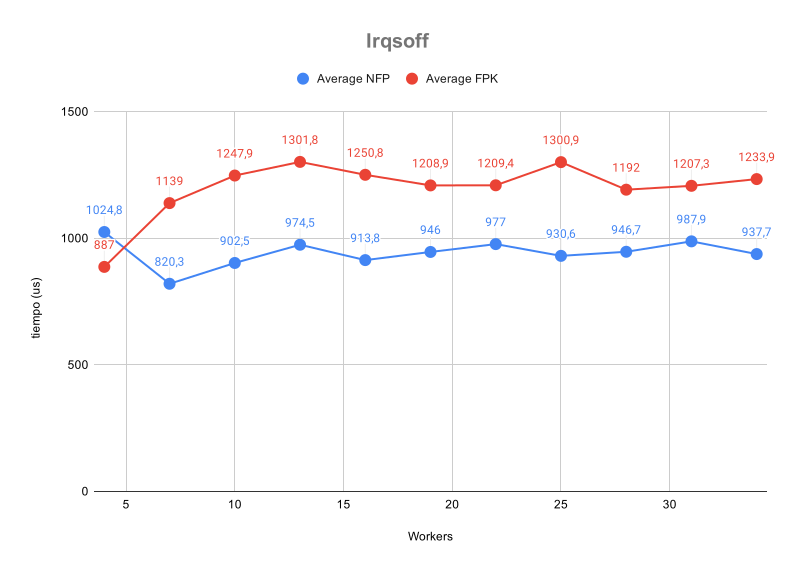
\includegraphics[width=15cm]{imagenes/graficas/Irqsoff.png}
    \caption{Gráfica comparativa de las medidas de irqsoff}
\end{figure}

%----------------------------------------------------------------------------------
\subsection{Latencia de planificación}

%--------------------------------------------------------------
\subsubsection{Latencia de planificación con tracer wakeup}

Los resultados agregados en una tabla son los siguientes:

% Please add the following required packages to your document preamble:
% \usepackage{multirow}
\begin{table}[htp]
\begin{tabular}{|c|c|c|c|c|c|c|c|c|}
\hline
\multicolumn{9}{|c|}{\textbf{scheduling (tracer wakeup)}}                                                                                                                            \\ \hline
\multirow{2}{*}{\textbf{nº workers}} & \multicolumn{4}{c|}{\textit{\textbf{No Forced Preemption}}}   & \multicolumn{4}{c|}{\textit{\textbf{Full Preemption}}}        \\ \cline{2-9} 
                                     & \textbf{Avg} & \textbf{Max} & \textbf{Min} & \textbf{Std Dev} & \textbf{Avg} & \textbf{Max} & \textbf{Min} & \textbf{Std Dev} \\ \hline
\textit{4}                           & 389,3        & 538          & 202          & 132,74           & 772,7        & 1296         & 456          & 251,54           \\ \hline
\textit{8}                           & 397,8        & 644          & 204          & 145,84           & 815,7        & 1147         & 675          & 143,76           \\ \hline
\textit{12}                          & 467,7        & 973          & 207          & 202,12           & 1128,5       & 1373         & 956          & 128,28           \\ \hline
\textit{16}                          & 1070,2       & 5557         & 200          & 1590,72          & 1359,3       & 1812         & 1126         & 228,47           \\ \hline
\textit{20}                          & 712,2        & 889          & 525          & 114,06           & 1459,2       & 1620         & 1179         & 118,31           \\ \hline
\textit{24}                          & 710,2        & 1020         & 437          & 189,56           & 1512,4       & 1698         & 1381         & 91,98            \\ \hline
\textit{28}                          & 759,9        & 1064         & 598          & 145,48           & 1578,8       & 1797         & 1424         & 130,53           \\ \hline
\textit{32}                          & 911,9        & 1219         & 573          & 211,92           & 1608,9       & 1742         & 1464         & 85,62            \\ \hline
\textit{36}                          & 746,5        & 1057         & 502          & 180,07           & 1820,5       & 2338         & 1446         & 288,11           \\ \hline
\textit{40}                          & 953,9        & 1438         & 491          & 287,21           & 1796,1       & 2179         & 1655         & 157,29           \\ \hline
\textit{44}                          & 1081,6       & 2437         & 668          & 504,39           & 1791,1       & 1895         & 1653         & 97,70            \\ \hline
\end{tabular}
\end{table}

Y se corresponden con esta gráfica:

\begin{figure}[htp]
    \centering
    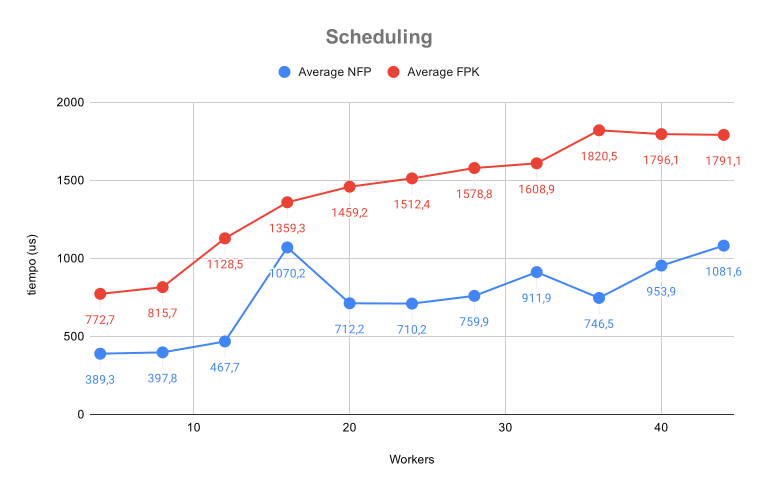
\includegraphics[width=15cm]{imagenes/graficas/Scheduling.png}
    \caption{Gráfica comparativa de las medidas de latencia de planificación usando el tracer wakeup}
\end{figure}

%--------------------------------------------------------------
\subsubsection{Latencia de planificación con filtros}

Los resultados agregados en una tabla son los siguientes:

% Please add the following required packages to your document preamble:
% \usepackage{multirow}
\begin{table}[htp]
\begin{tabular}{|c|c|c|c|c|c|c|c|c|}
\hline
\multicolumn{9}{|c|}{\textbf{scheduling (filtros)}}                                                                                                                     \\ \hline
\multirow{2}{*}{\textbf{nº workers}} & \multicolumn{4}{c|}{\textit{\textbf{No Forced Preemption}}}   & \multicolumn{4}{c|}{\textit{\textbf{Full Preemption}}}        \\ \cline{2-9} 
                                     & \textbf{Avg} & \textbf{Max} & \textbf{Min} & \textbf{Std Dev} & \textbf{Avg} & \textbf{Max} & \textbf{Min} & \textbf{Std Dev} \\ \hline
\textit{4}                           & 35.525       & 42.040       & 28.744       & 5234,18          & 41.053       & 44.506       & 33.081       & 3518,25          \\ \hline
\textit{8}                           & 44.260       & 53.979       & 34.509       & 5227,03          & 46.738       & 51.147       & 42.527       & 2482,41          \\ \hline
\textit{12}                          & 68.137       & 92.789       & 48.091       & 13179,34         & 61.326       & 70.424       & 53.535       & 4888,50          \\ \hline
\textit{16}                          & 87.994       & 99.728       & 73.820       & 8181,93          & 72.344       & 77.025       & 69.036       & 2791,62          \\ \hline
\textit{20}                          & 115.398      & 133.612      & 91.740       & 13953,35         & 92.517       & 106.393      & 78.061       & 8805,40          \\ \hline
\textit{24}                          & 180.121      & 206.602      & 168.037      & 13399,69         & 122.896      & 165.050      & 101.291      & 18812,36         \\ \hline
\textit{28}                          & 227.553      & 250.089      & 190.498      & 21691,67         & 177.471      & 210.512      & 149.200      & 17820,29         \\ \hline
\textit{32}                          & 282.802      & 302.741      & 251.664      & 17189,56         & 251.706      & 286.793      & 229.608      & 22079,15         \\ \hline
\textit{36}                          & 358.032      & 369.510      & 337.391      & 10478,38         & 413.173      & 706.037      & 300.010      & 145870,54        \\ \hline
\textit{40}                          & 415.128      & 430.815      & 394.227      & 13862,23         & 425.685      & 448.892      & 407.551      & 13829,08         \\ \hline
\textit{44}                          & 487.172      & 507.610      & 447.544      & 18537,60         & 513.896      & 556.127      & 492.790      & 20518,42         \\ \hline
\end{tabular}
\end{table}

Y se corresponden con esta gráfica:

\begin{figure}[htp]
    \centering
    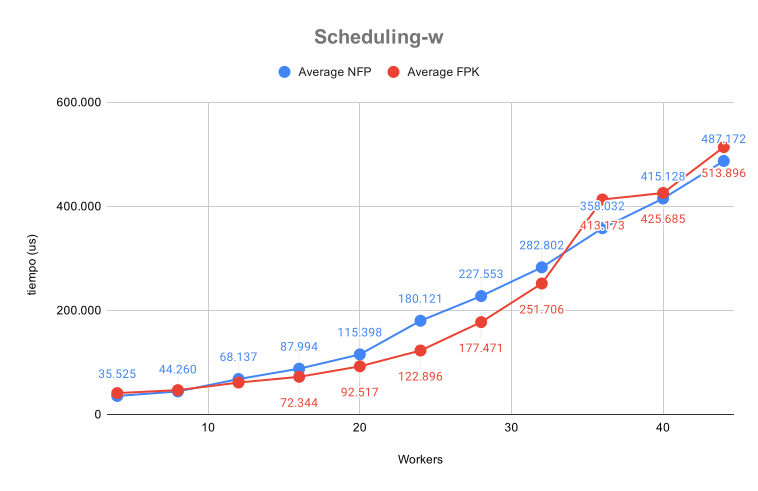
\includegraphics[width=15cm]{imagenes/graficas/Scheduling-w.png}
    \caption{Gráfica comparativa de las medidas de latencia de planificación usando filtros}
\end{figure}


%----------------------------------------------------------------------------------
\subsection{Latencia de llamada al sistema}

Los resultados agregados en una tabla son los siguientes:

% Please add the following required packages to your document preamble:
% \usepackage{multirow}
\begin{table}[htp]
\begin{tabular}{|c|c|c|c|c|c|c|c|c|}
\hline
\multicolumn{9}{|c|}{\textbf{syscalls}}                                                                                                                              \\ \hline
\multirow{2}{*}{\textbf{nº workers}} & \multicolumn{4}{c|}{\textit{\textbf{No Forced Preemption}}}   & \multicolumn{4}{c|}{\textit{\textbf{Full Preemption}}}        \\ \cline{2-9} 
                                     & \textbf{Avg} & \textbf{Max} & \textbf{Min} & \textbf{Std Dev} & \textbf{Avg} & \textbf{Max} & \textbf{Min} & \textbf{Std Dev} \\ \hline
\textit{1}                           & 301,8        & 419          & 121          & 137,80           & 475          & 607          & 450          & 46,81            \\ \hline
\textit{3}                           & 1172,5       & 2351         & 232          & 839,34           & 2574,8       & 2907         & 2335         & 158,35           \\ \hline
\textit{5}                           & 3334,2       & 4005         & 903          & 1281,95          & 4520,2       & 4753         & 4442         & 110,38           \\ \hline
\textit{7}                           & 4602         & 4614         & 4575         & 11,26            & 6640         & 6887         & 5996         & 293,32           \\ \hline
\textit{9}                           & 5980,4       & 6007         & 5926         & 24,16            & 8763         & 8881         & 8525         & 122,28           \\ \hline
\textit{11}                          & 7369,6       & 7410         & 7344         & 24,40            & 10811,4      & 10918        & 10587        & 96,72            \\ \hline
\textit{13}                          & 8730,2       & 8751         & 8712         & 14,10            & 12717,4      & 12905        & 12418        & 163,14           \\ \hline
\textit{15}                          & 10083,8      & 10144        & 10005        & 46,36            & 14579,9      & 14812        & 14055        & 267,78           \\ \hline
\textit{17}                          & 11421,9      & 11483        & 11325        & 51,61            & 16628,1      & 16744        & 16458        & 100,14           \\ \hline
\textit{19}                          & 12800,9      & 13096        & 12734        & 106,50           & 18512,6      & 18711        & 18322        & 118,34           \\ \hline
\textit{21}                          & 14117,3      & 14286        & 13991        & 103,82           & 20288,5      & 20552        & 19892        & 202,95           \\ \hline
\end{tabular}
\end{table}

Y se corresponden con esta gráfica:

\begin{figure}[htp]
    \centering
    \includegraphics[width=15cm]{imagenes/graficas/Syscall-write.png}
    \caption{Gráfica comparativa de las medidas de latencia de llamada al sistema}
\end{figure}


\end{document}
